\documentclass{article}
\usepackage[utf8]{inputenc}
\usepackage{amsmath}
\usepackage{graphicx}
\usepackage{booktabs}
\usepackage{caption}
\usepackage{adjustbox}


\title{Informe de Análisis Exploratorio de \texttt{swiss}}
\author{
  Melani Forsythe Matos \\
  Daniela Guerrero Álvarez \\
  Rubén Martínez Rojas
}
\date{} % Sin fecha para que no aparezca
\begin{document}

\maketitle









\section{Introducción}
El dataset ``swiss'' contiene datos sobre 47 cantones suizos en 1888. Este análisis proporciona una visión detallada de las variables relacionadas con la fertilidad, la agricultura, y la educación.

\section{Descripción de las Variables}
El dataset ``swiss'' incluye las siguientes variables:
\begin{itemize}
    \item \textbf{Fertility}: Tasa de fertilidad (número de hijos por mujer).
    \item \textbf{Agriculture}: Proporción de trabajadores en agricultura.
    \item \textbf{Examination}: Proporción de jóvenes con educación secundaria.
    \item \textbf{Education}: Proporción de población con educación secundaria.
    \item \textbf{Catholic}: Proporción de población católica.
    \item \textbf{Infant.Mortality}: Tasa de mortalidad infantil (número de muertes por 1000 nacidos vivos).
\end{itemize}

\section*{Análisis Descriptivo}

1. \textbf{Fertility}:
\begin{figure}[h!]
 \centering
 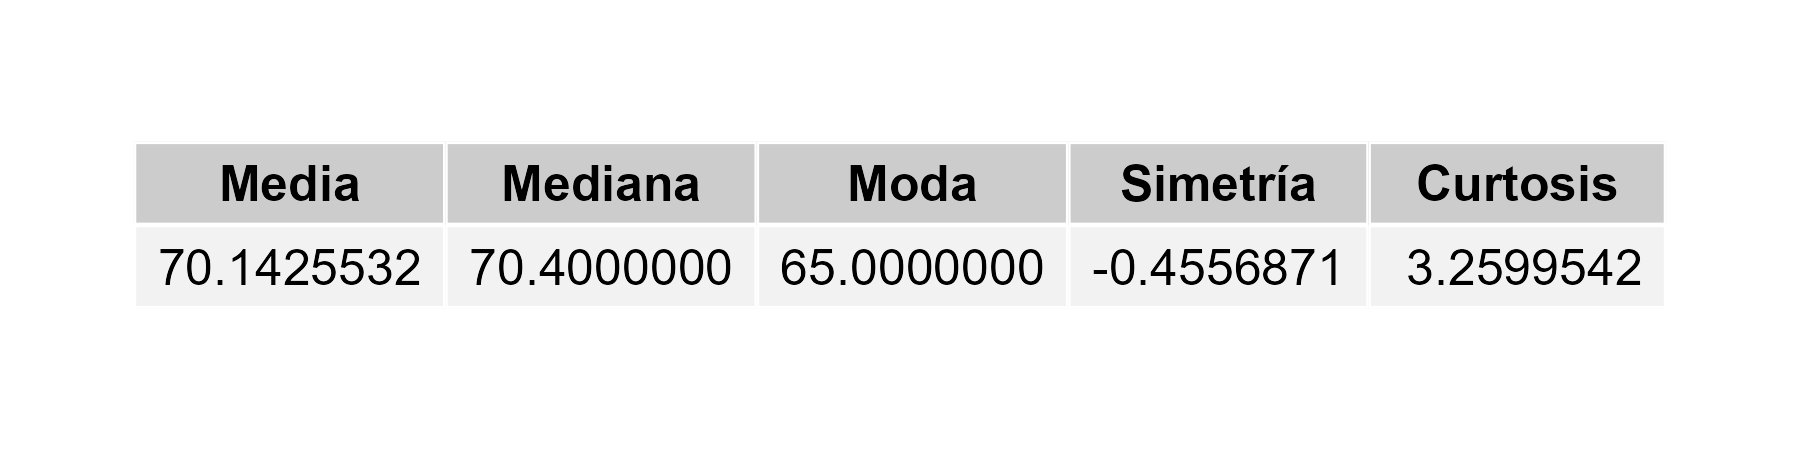
\includegraphics[width=\textwidth]{Swiss/Fertility_central.png}
 \caption{Medidas centrales de Fertilidad}
\end{figure}

\begin{figure}[h!]
 \centering
 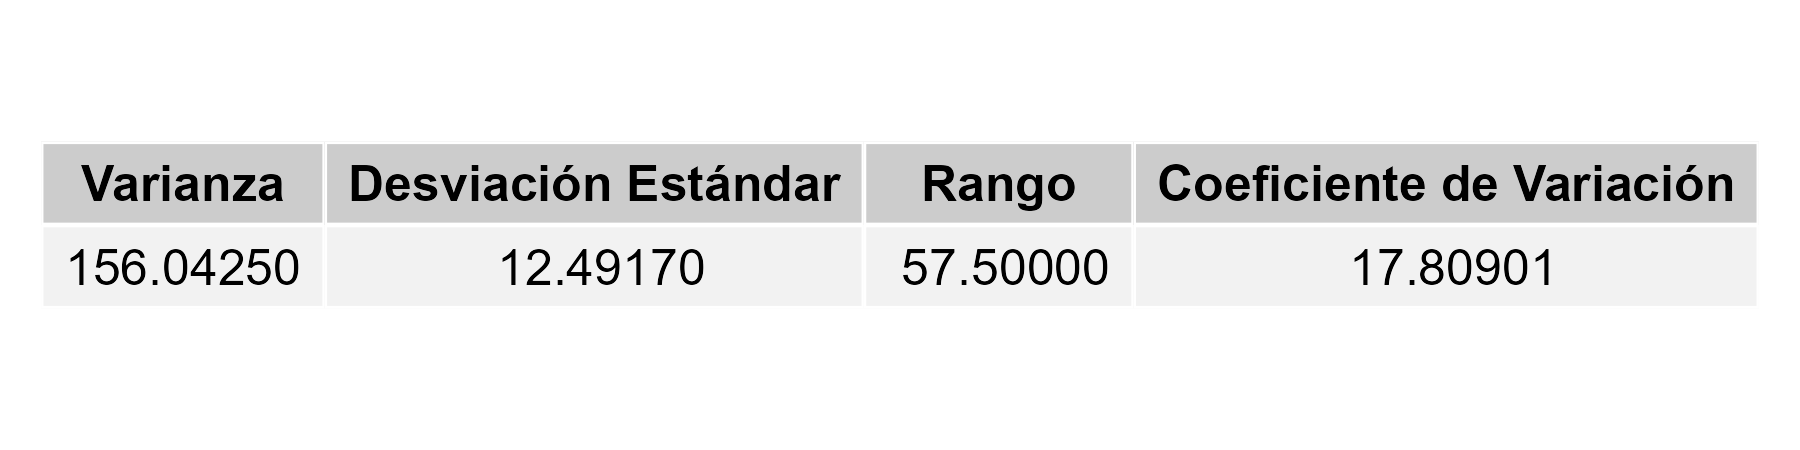
\includegraphics[width=\textwidth]{Swiss/Fertility_dispersion.png}
 \caption{Medidas de dispersión de Fertilidad}
\end{figure}

   \begin{itemize}
       \item La media es 70.14, indicando el promedio del índice de fertilidad.
       \item La mediana es 70.4, lo que sugiere que la mitad de los valores están por debajo de este nivel.
       \item La moda es 65, el valor más frecuente en los datos de fertilidad.
       \item La simetría negativa (-0.46) sugiere una ligera inclinación hacia la izquierda, lo que implica que hay más valores altos que bajos.
       \item La curtosis de 3.26 indica una distribución ligeramente más apuntada que una distribución normal.
       \item La varianza es 156.04, reflejando una dispersión moderada de los datos.
       \item La desviación estándar es 12.49, mostrando una variabilidad significativa en los índices de fertilidad.
       \item El rango es 57.5, lo que indica una diferencia considerable entre el valor más alto y el más bajo.
       \item El coeficiente de variación es 17.81, lo que indica una variabilidad del 17.8\% respecto a la media.
   \end{itemize}

   \begin{figure}[h!]
    \centering
    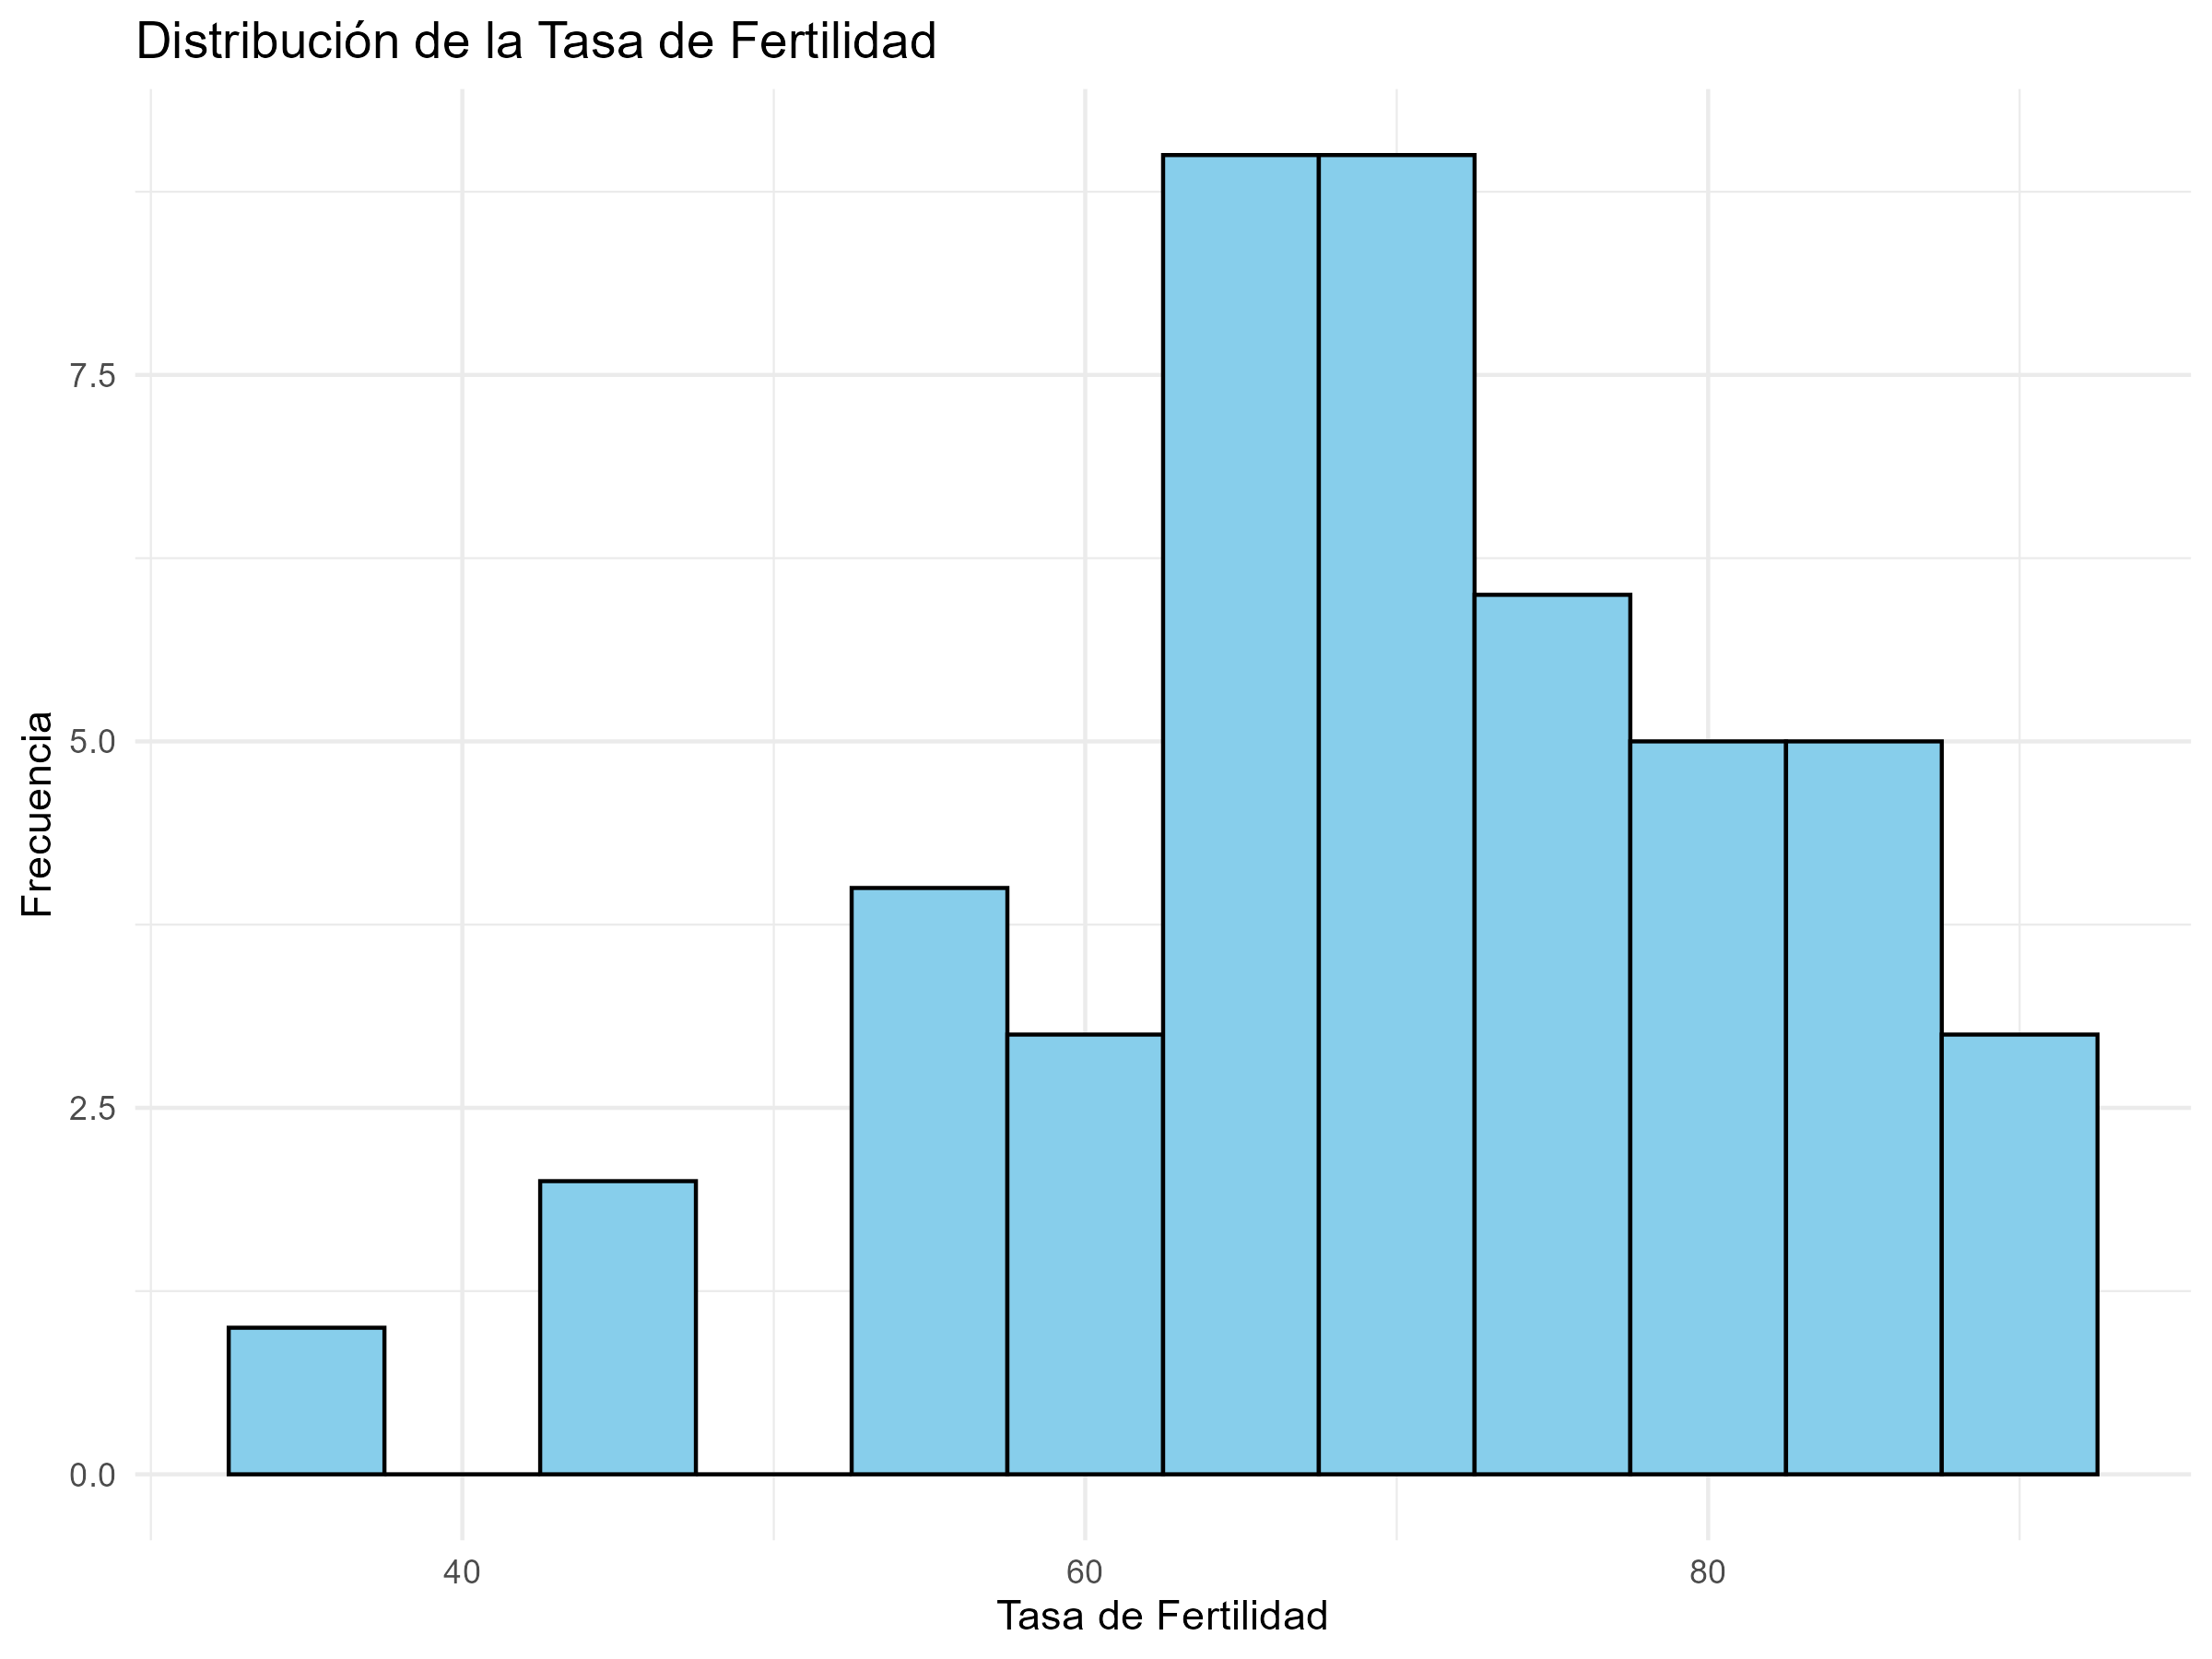
\includegraphics[width=\textwidth]{Histogramas/histogram_fertility.png}
    \caption{Distribución de la Tasa de Fertilidad}
    \end{figure}

2. \textbf{Agriculture}:
\begin{figure}[h!]
    \centering
    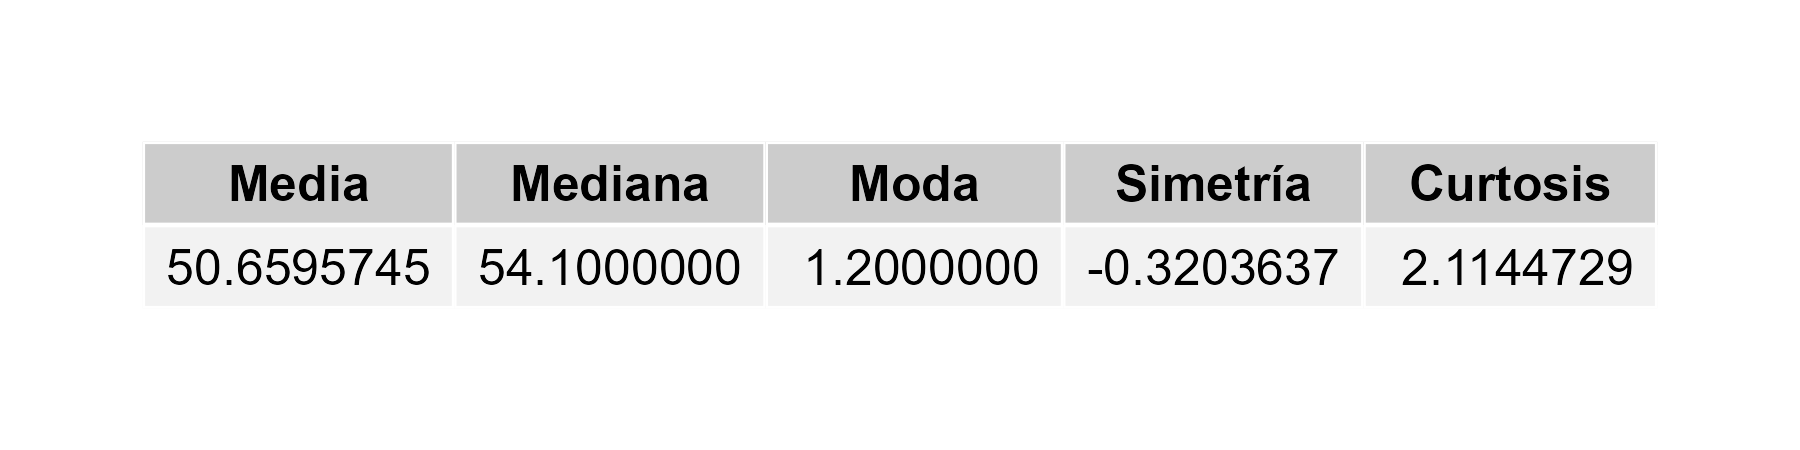
\includegraphics[width=\textwidth]{Swiss/Agriculture_central.png}
    \caption{Medidas centrales de Agricultura}
\end{figure}

\begin{figure}[h!]
    \centering
    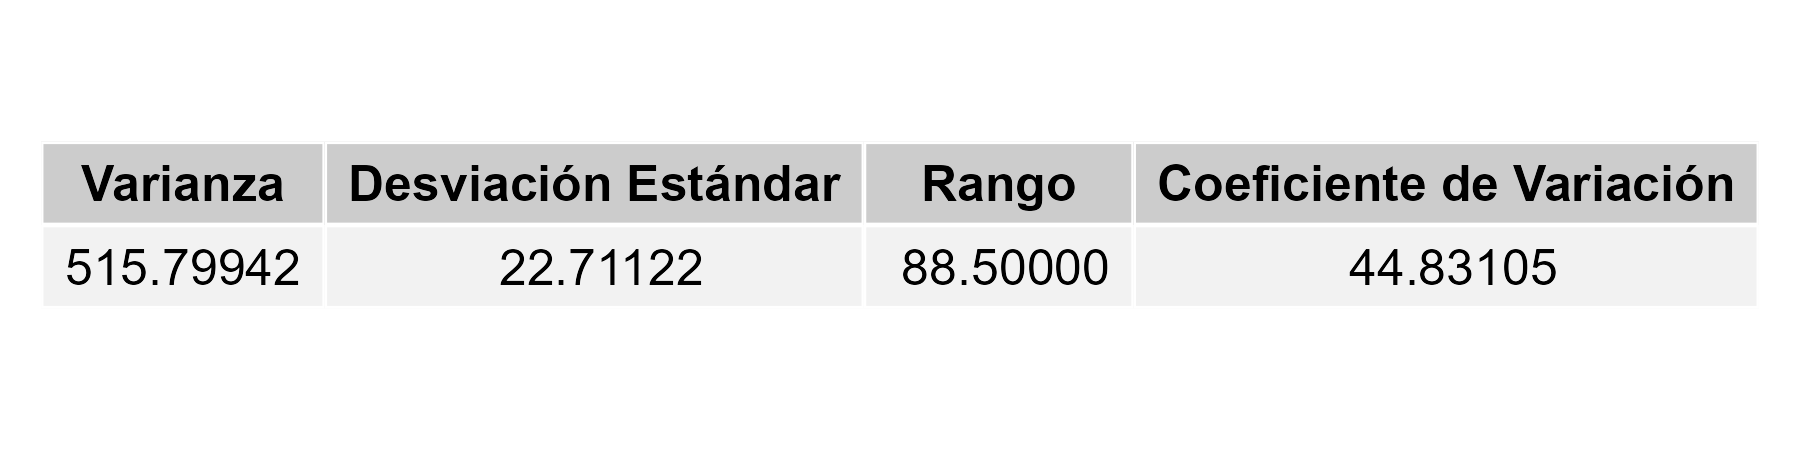
\includegraphics[width=\textwidth]{Swiss/Agriculture_dispersion.png}
    \caption{Medidas de dispersión de Agricultura}
\end{figure}
\begin{itemize}
    \item La media es 50.66, lo que representa el porcentaje promedio de personas dedicadas a la agricultura.
       \item La mediana es 54.1, lo que sugiere que la mitad de las observaciones tienen un valor menor o igual a 54.1.
       \item La moda es 1.2, el valor más común en los datos de agricultura.
       \item La simetría negativa (-0.32) indica una ligera inclinación hacia la izquierda.
       \item La curtosis de 2.11 sugiere una distribución algo más plana en comparación con una distribución normal.
       \item La varianza es 515.8, reflejando una alta dispersión en los datos de agricultura.
       \item La desviación estándar es 22.71, mostrando una alta variabilidad respecto a la media.
       \item El rango es 88.5, indicando una gran diferencia entre el valor más alto y el más bajo.
       \item El coeficiente de variación es 44.83, lo que indica una alta variabilidad respecto a la media.
   \end{itemize}


       \begin{figure}[h!]
        \centering
        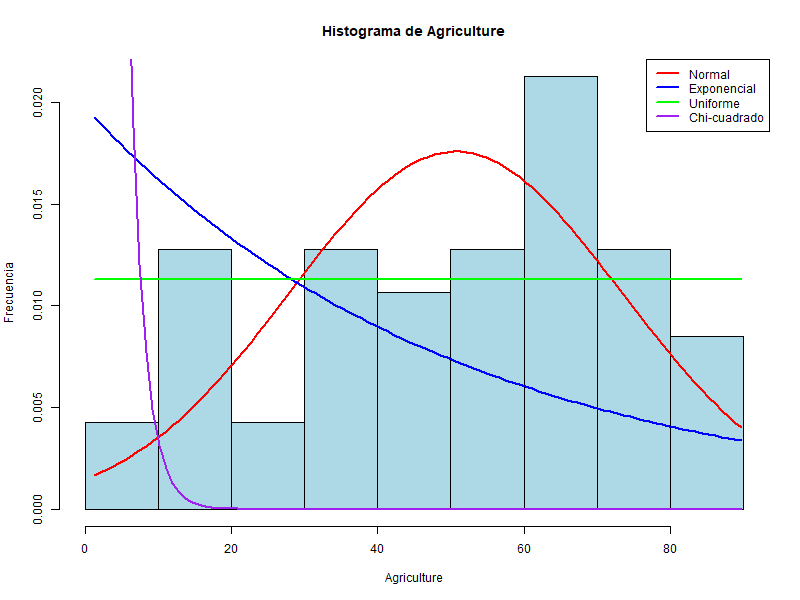
\includegraphics[width=\textwidth]{Histogramas/histogram_agriculture.png}
        \caption{Distribución de la Proporción de Trabajadores en Agricultura}
        \end{figure}
   
   3. \textbf{Examination}:
   \begin{figure}[h!]
 \centering
 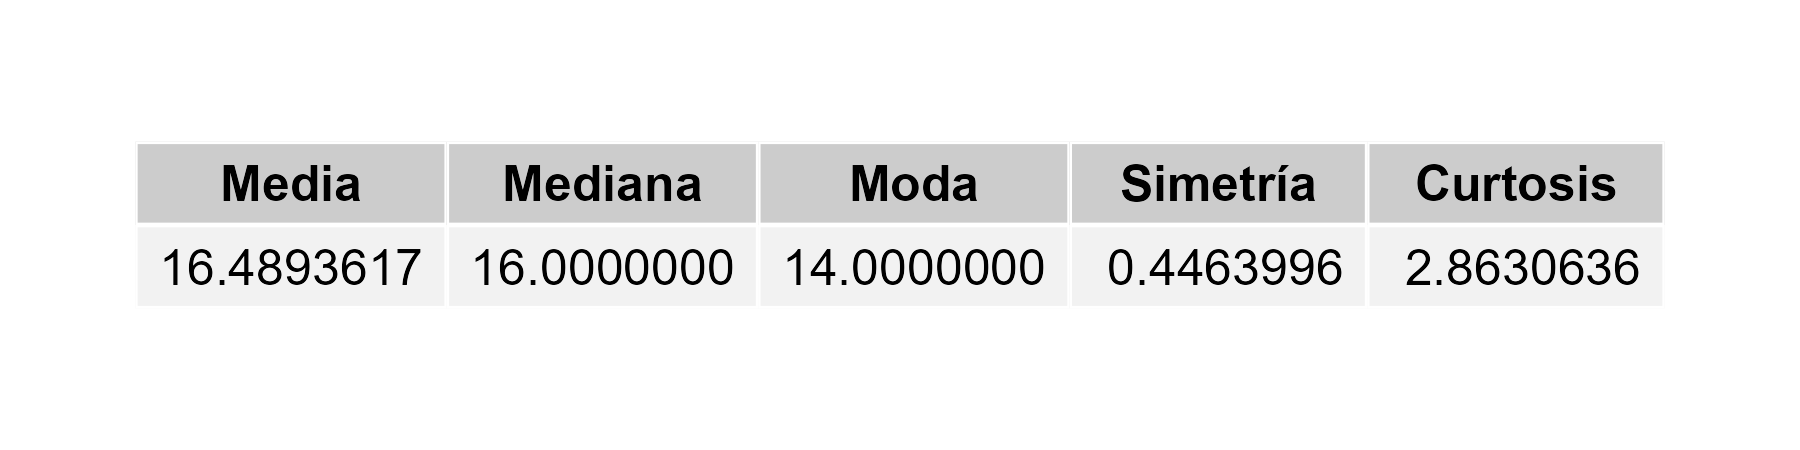
\includegraphics[width=\textwidth]{Swiss/Examination_central.png}
 \caption{Medidas centrales de Exámenes}
\end{figure}

\begin{figure}[h!]
 \centering
 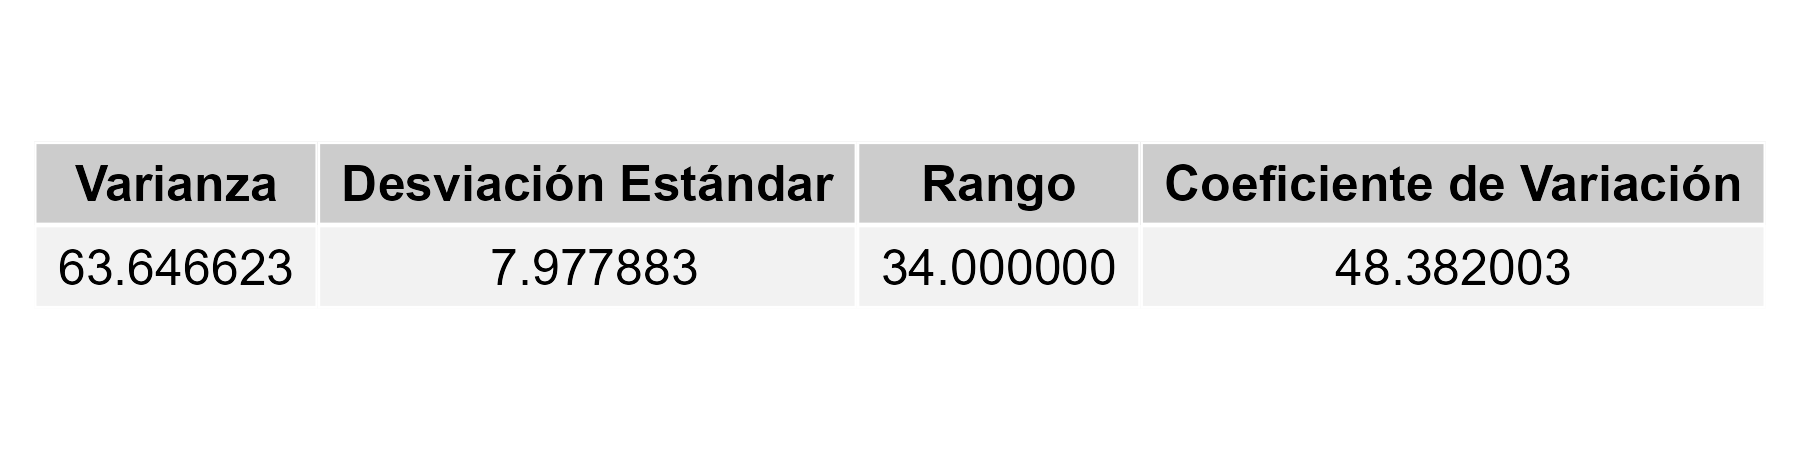
\includegraphics[width=\textwidth]{Swiss/Examination_dispersion.png}
 \caption{Medidas de dispersión de Exámenes}
\end{figure}
   \begin{itemize}
       \item La media es 16.49, representando el promedio de la tasa de aprobación en exámenes.
       \item La mediana es 16, lo que sugiere que la mitad de los valores están por debajo de este nivel.
       \item La moda es 14, el valor más frecuente.
       \item La simetría positiva (0.45) sugiere una ligera inclinación hacia la derecha.
       \item La curtosis de 2.86 indica una distribución ligeramente más apuntada que la normal.
       \item La varianza es 63.65, reflejando una dispersión considerable.
       \item La desviación estándar es 7.98, indicando una variabilidad moderada.
       \item El rango es 34, reflejando una gran diferencia entre el valor más alto y el más bajo.
       \item El coeficiente de variación es 48.38, lo que indica una alta variabilidad respecto a la media.
   \end{itemize}

   \begin{figure}[h!]
    \centering
    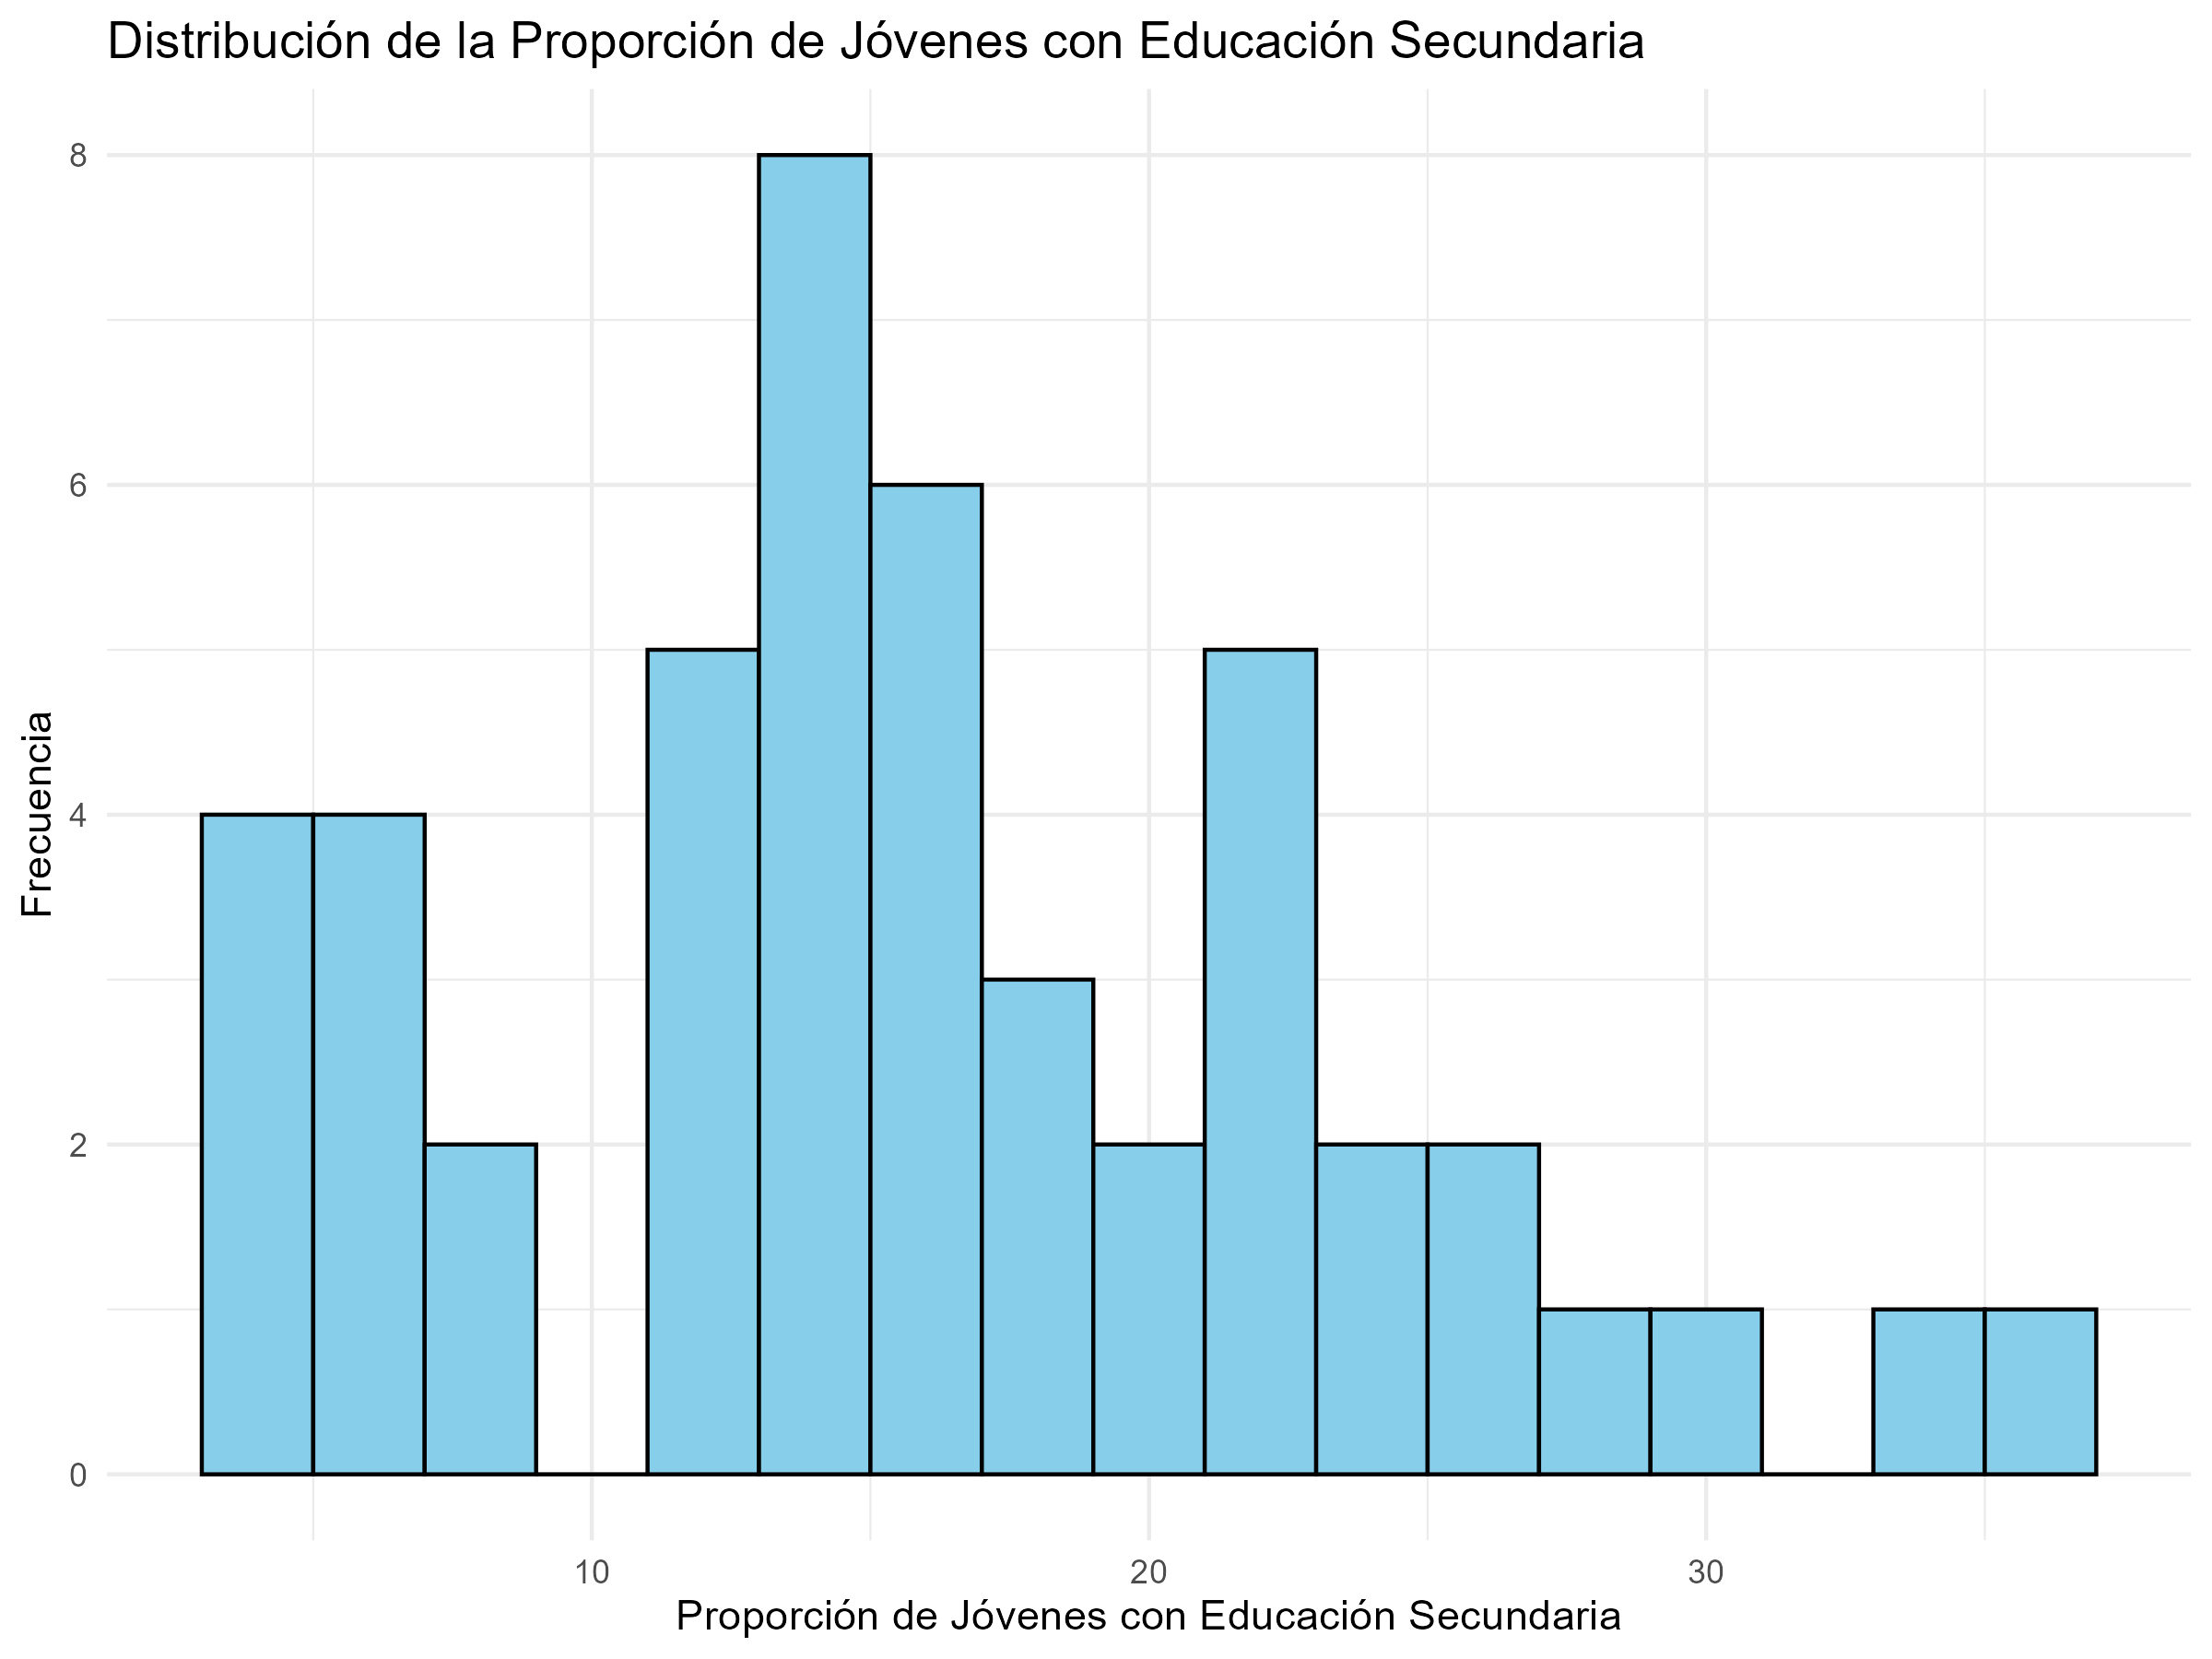
\includegraphics[width=\textwidth]{Histogramas/histogram_examination.png}
    \caption{Distribución de la Proporción de Jóvenes con Educación Secundaria}
    \end{figure}

4. \textbf{Education}:

   \begin{figure}[h!]
    \centering
    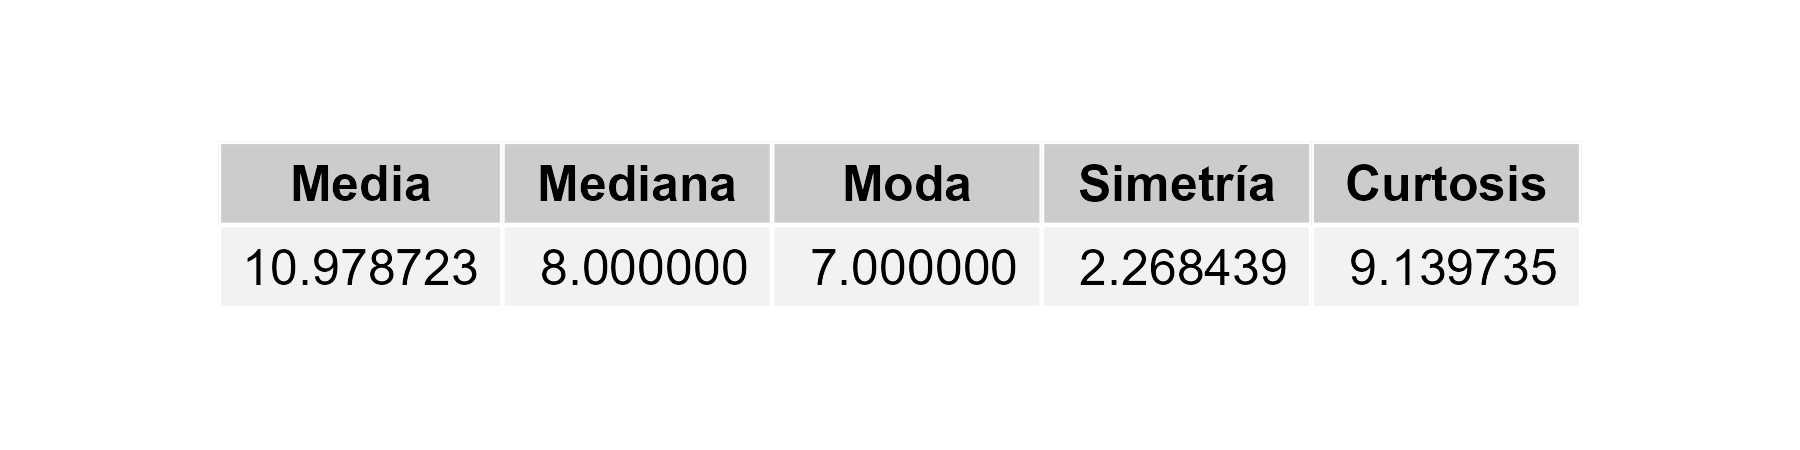
\includegraphics[width=\textwidth]{Swiss/Education_central.png}
    \caption{Medidas centrales de Educación}
\end{figure}

\begin{figure}[h!]
    \centering
    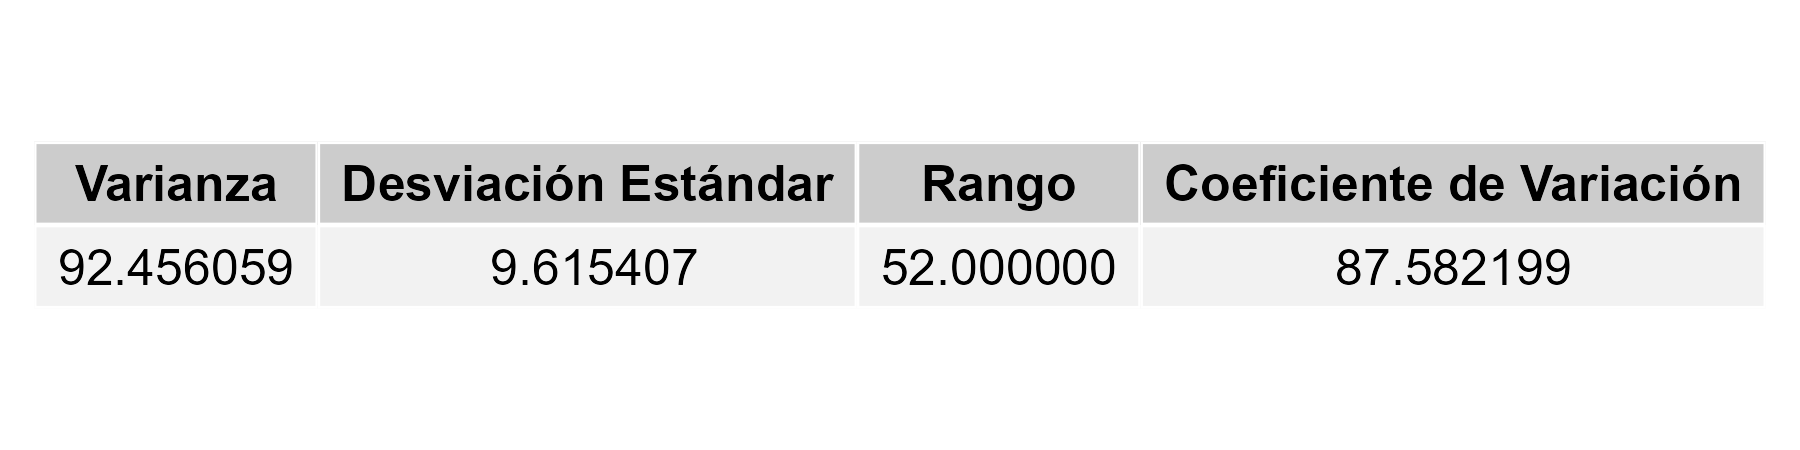
\includegraphics[width=\textwidth]{Swiss/Education_dispersion.png}
    \caption{Medidas de dispersión de Educación}
\end{figure}
   \begin{itemize}
       \item La media es 10.98, lo que indica el promedio del nivel de educación.
       \item La mediana es 8, sugiriendo que la mitad de los valores están por debajo de este nivel.
       \item La moda es 7, el valor más frecuente.
       \item La simetría positiva (2.27) indica una fuerte inclinación hacia la derecha, con una cola larga hacia los valores altos.
       \item La curtosis de 9.14 sugiere una distribución extremadamente apuntada.
       \item La varianza es 92.46, reflejando una dispersión considerable en los niveles de educación.
       \item La desviación estándar es 9.62, mostrando una alta variabilidad.
       \item El rango es 52, reflejando una gran diferencia entre el valor más alto y el más bajo.
       \item El coeficiente de variación es 87.58, indicando una variabilidad muy alta respecto a la media.
   \end{itemize}

   \begin{figure}[h!]
    \centering
    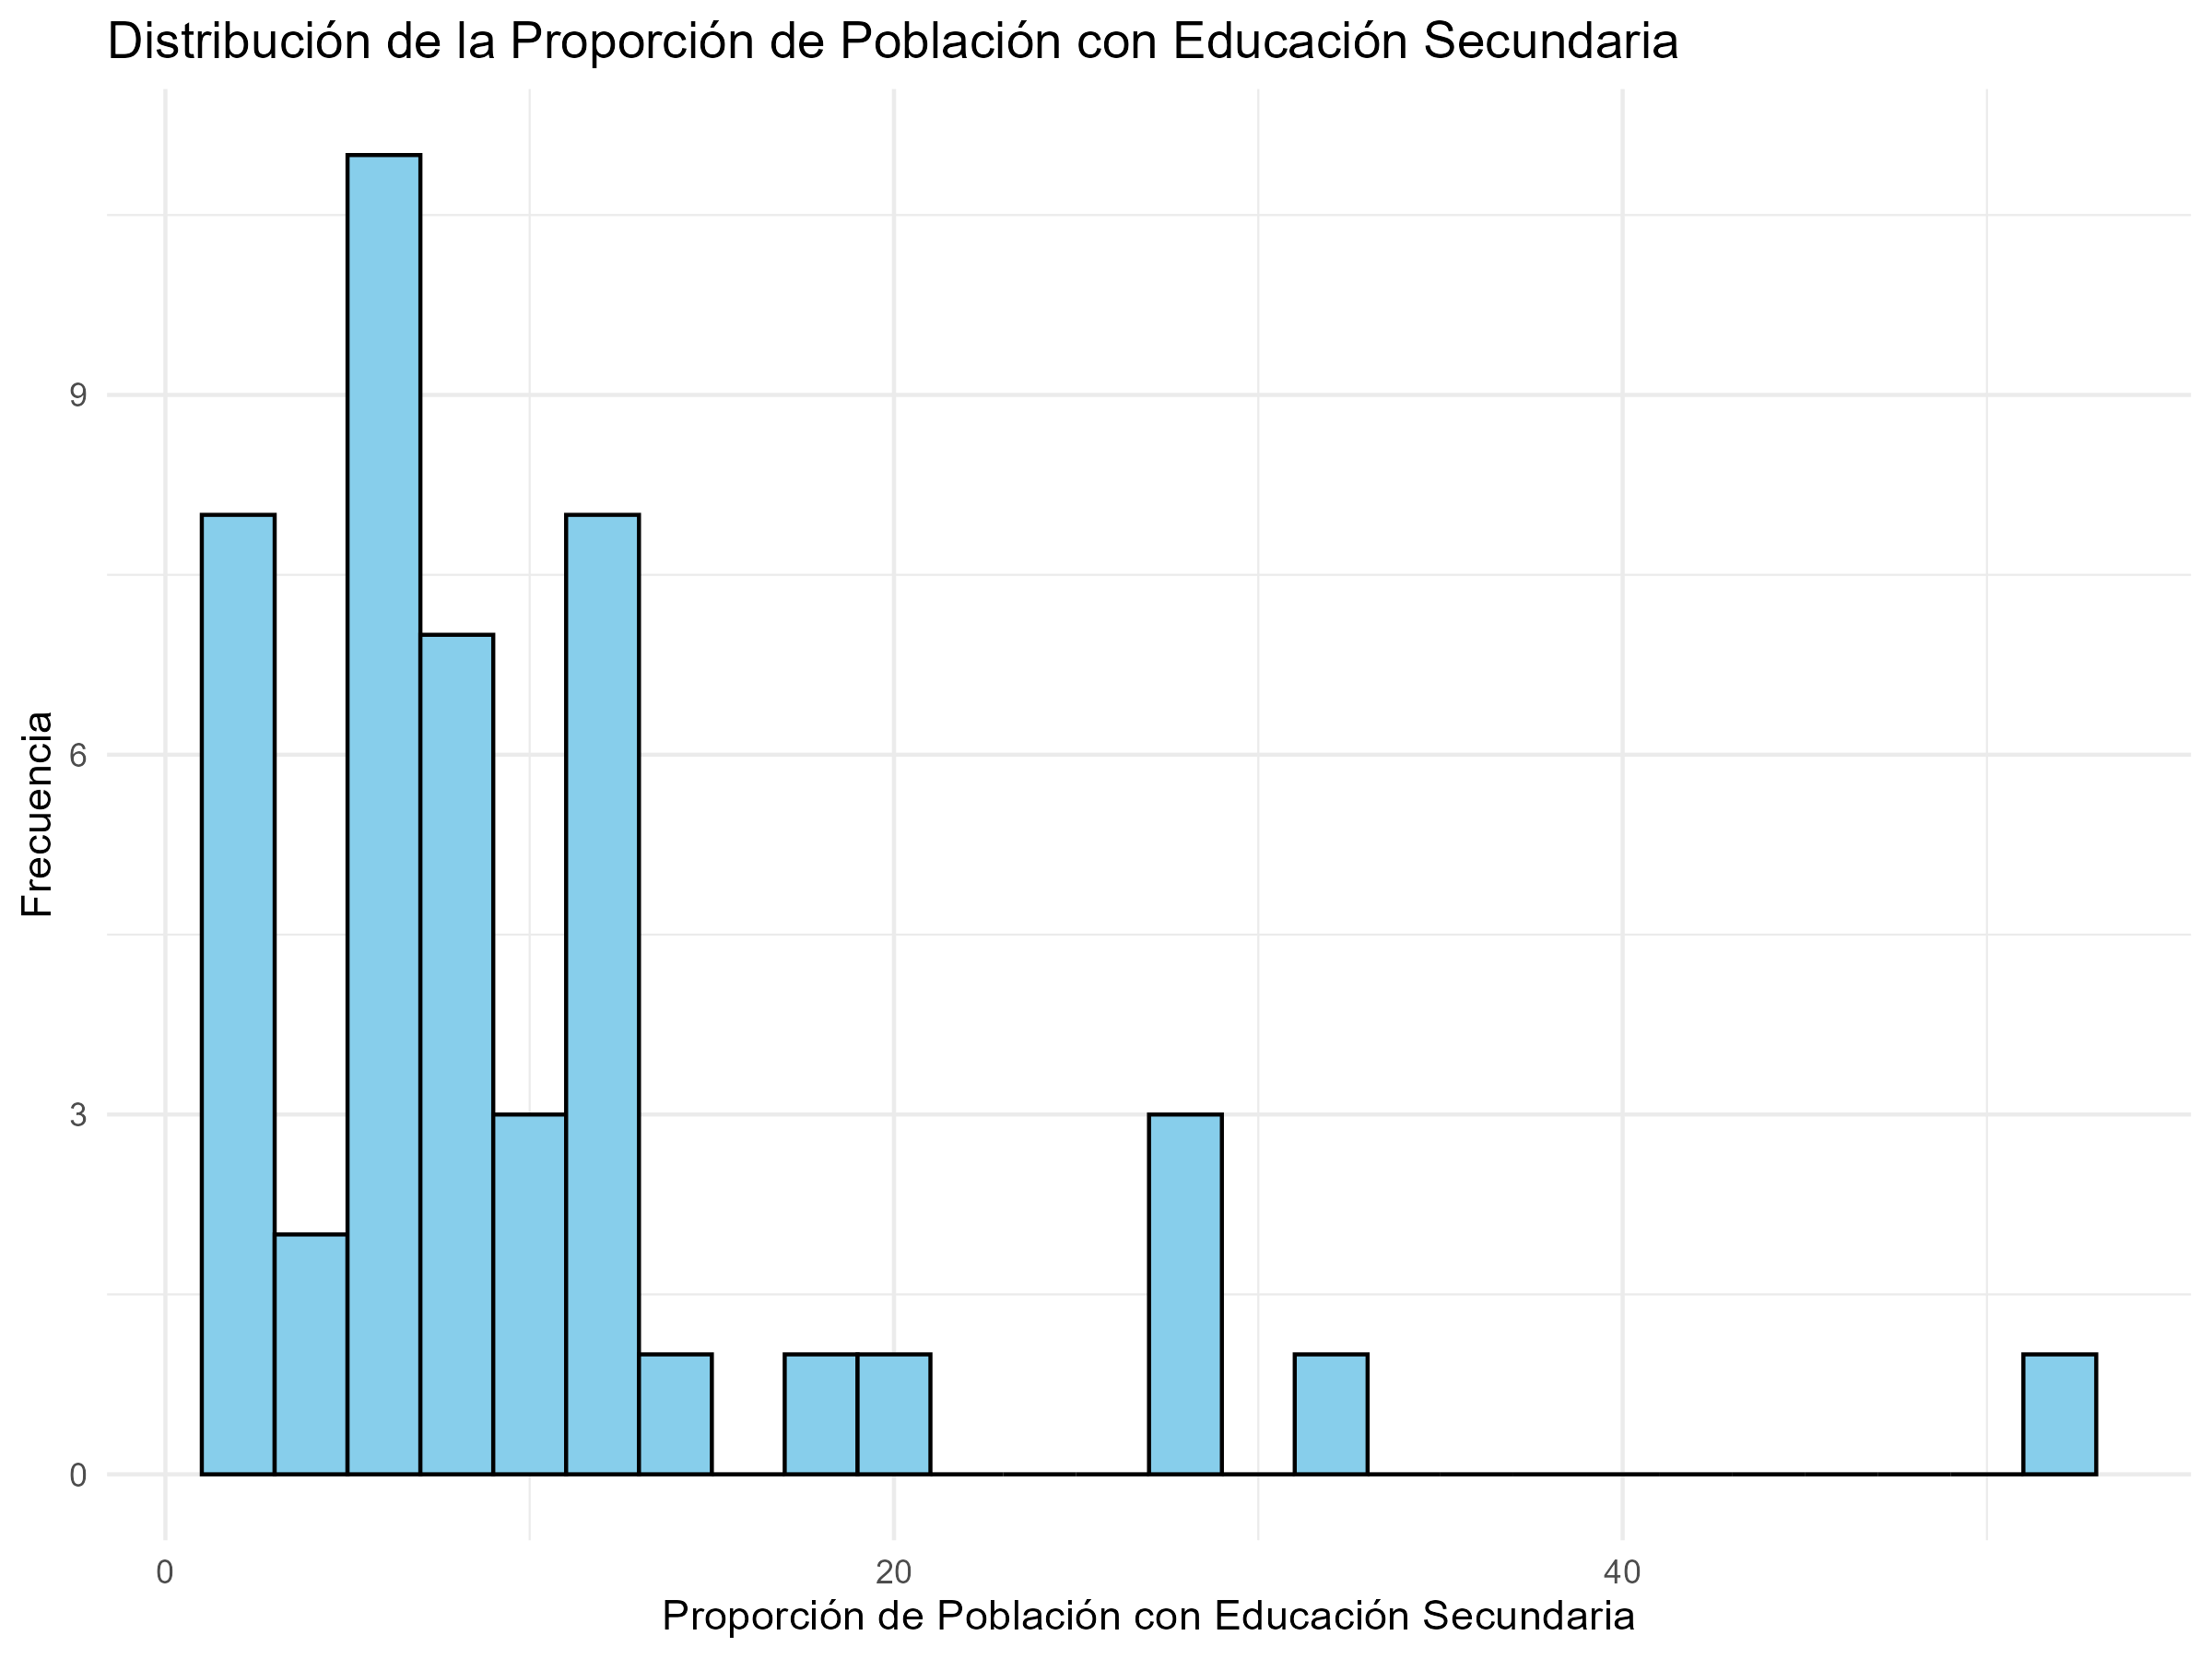
\includegraphics[width=\textwidth]{Histogramas/histogram_education.png}
    \caption{Distribución de la Proporción de Población con Educación Secundaria}
    \end{figure}

5. \textbf{Catholic}:
\begin{figure}[h!]
 \centering
 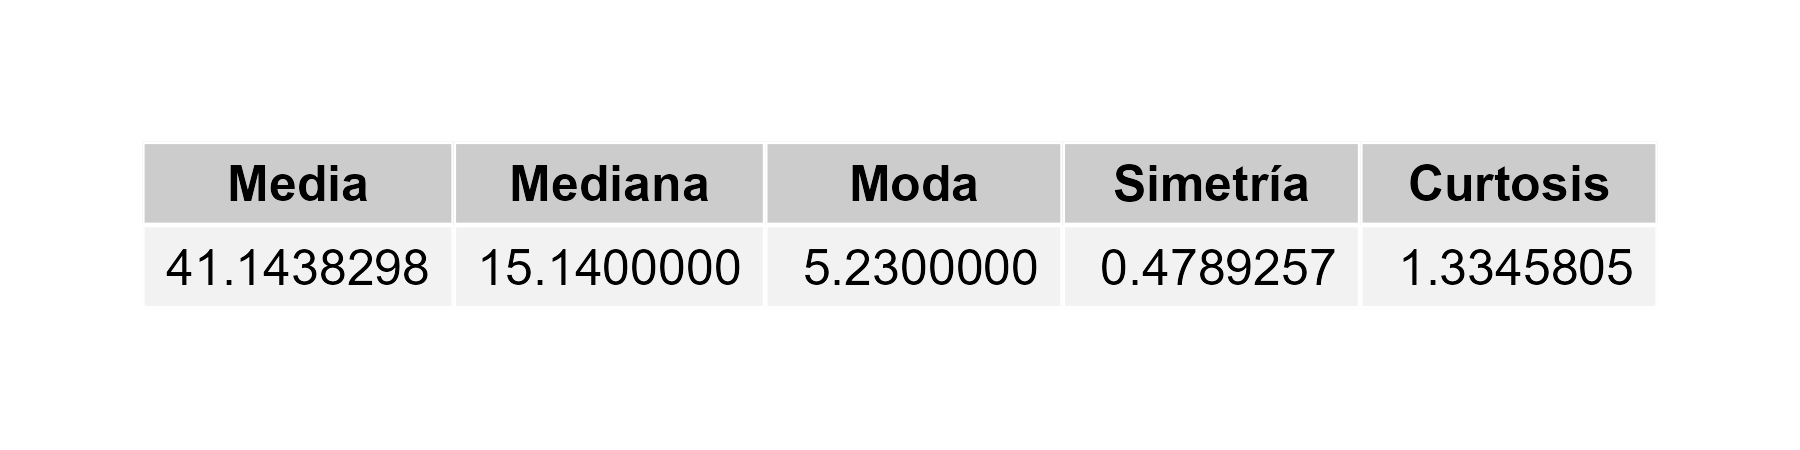
\includegraphics[width=\textwidth]{Swiss/Catholic_central.png}
 \caption{Medidas centrales de Población Católica}
\end{figure}

\begin{figure}[h!]
 \centering
 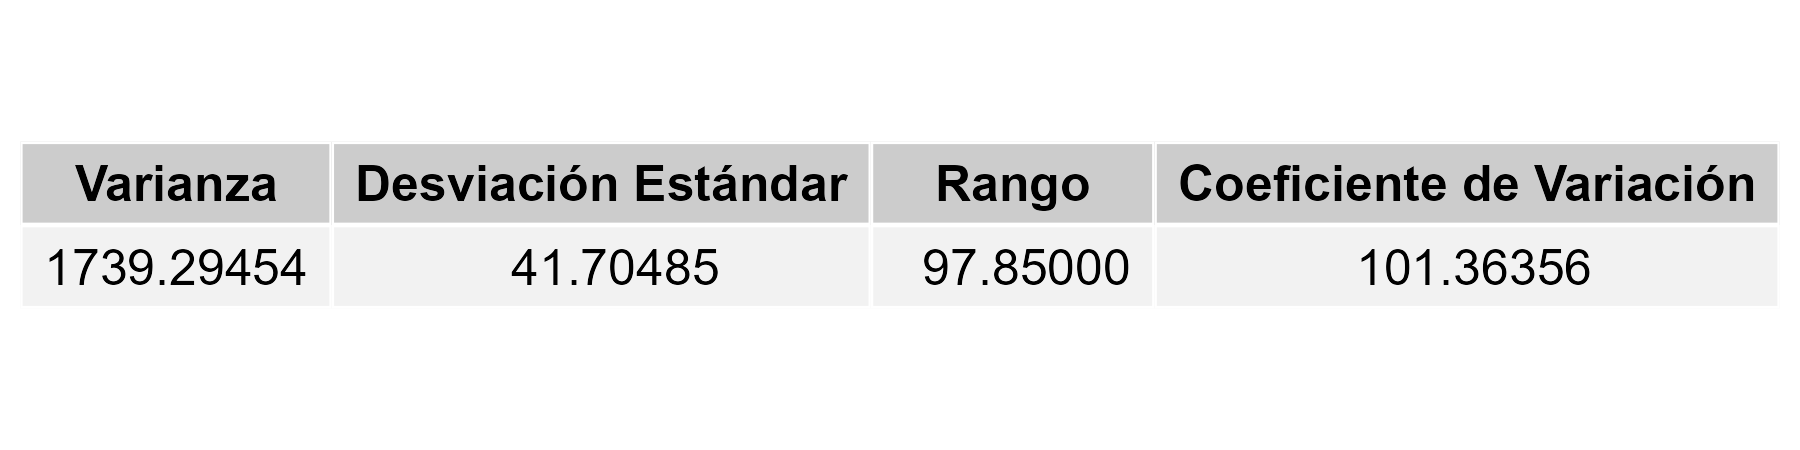
\includegraphics[width=\textwidth]{Swiss/Catholic_dispersion.png}
 \caption{Medidas de dispersión de Población Católica}
\end{figure}
   \begin{itemize}
       \item La media es 41.14, representando el porcentaje promedio de población católica.
       \item La mediana es 15.14, lo que sugiere que la mitad de las observaciones están por debajo de este valor.
       \item La moda es 5.23, el valor más común.
       \item La simetría positiva (0.48) indica una ligera inclinación hacia la derecha.
       \item La curtosis de 1.33 indica una distribución más plana que una distribución normal.
       \item La varianza es 1739.29, reflejando una dispersión extremadamente alta en los porcentajes de población católica.
       \item La desviación estándar es 41.70, mostrando una gran variabilidad.
       \item El rango es 97.85, lo que refleja una gran diferencia entre el valor más alto y el más bajo.
       \item El coeficiente de variación es 101.36, lo que indica una variabilidad extremadamente alta respecto a la media.
   \end{itemize}

   \begin{figure}[h!]
    \centering
    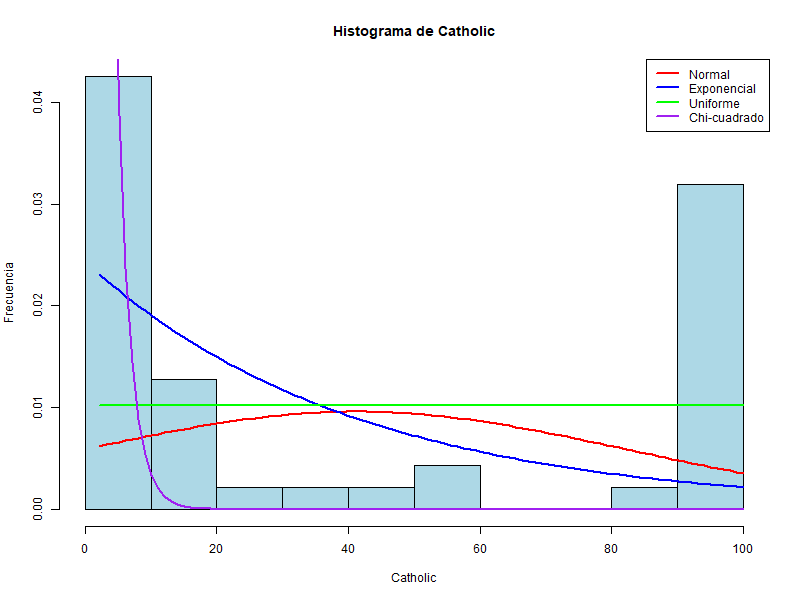
\includegraphics[width=\textwidth]{Histogramas/histogram_catholic.png}
    \caption{Distribución de la Proporción de Población Católica}
    \end{figure}


6. \textbf{Infant Mortality}:
\begin{figure}[h!]
 \centering
 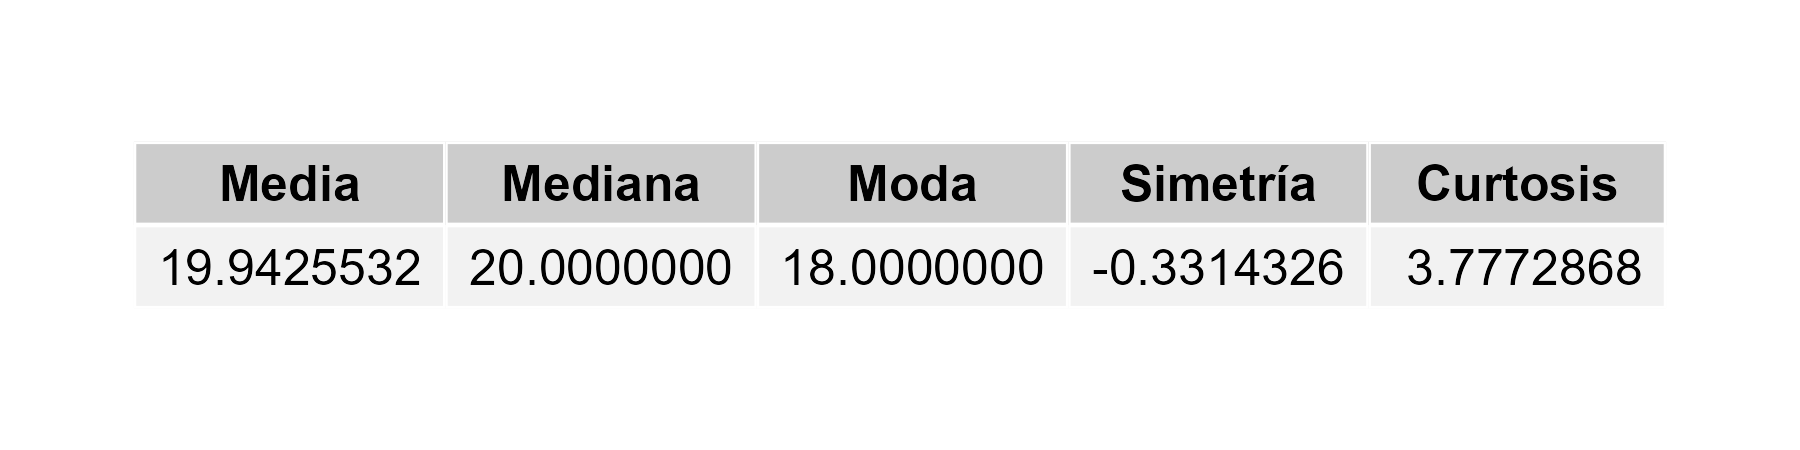
\includegraphics[width=\textwidth]{Swiss/Infant.Mortality_central.png}
 \caption{Medidas centrales de Mortalidad Infantil}
\end{figure}

\begin{figure}[h!]
    \centering
    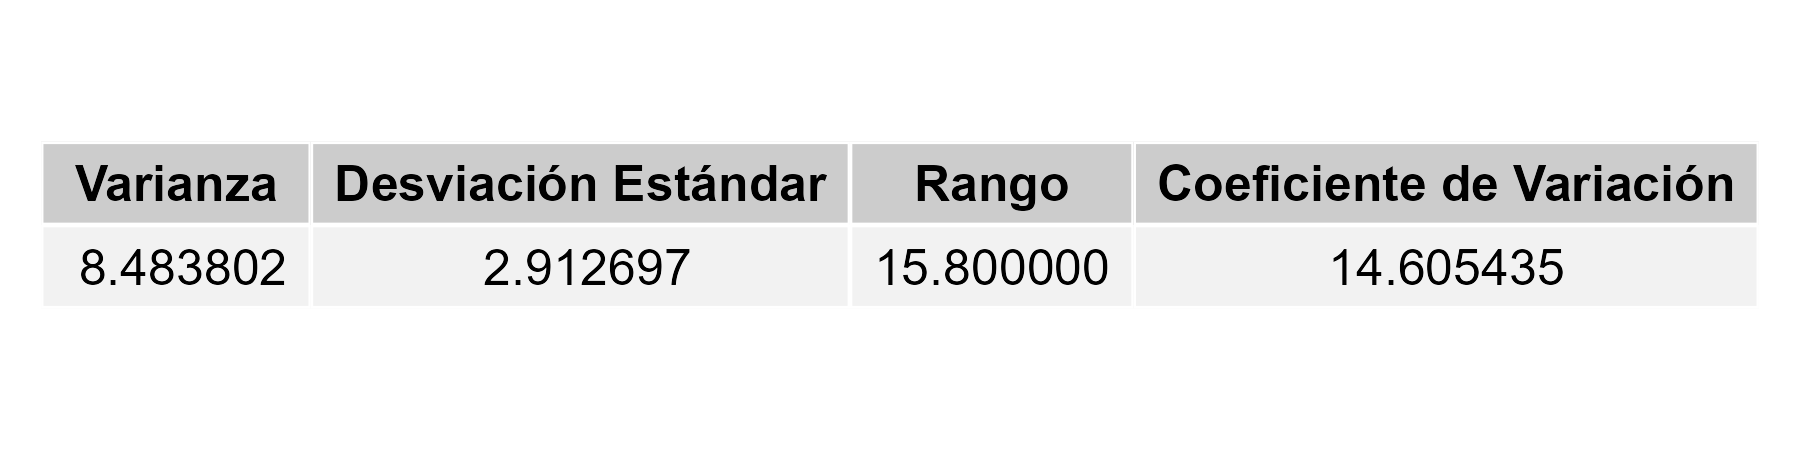
\includegraphics[width=\textwidth]{Swiss/Infant.Mortality_dispersion.png}
    \caption{Medidas de dispersión de Mortalidad Infantil}
\end{figure}
\begin{itemize}
    \item La media es 19.94, lo que indica el promedio de la tasa de mortalidad infantil.
    \item La mediana es 20, lo que sugiere que la mitad de los valores están por debajo de este nivel.
    \item La moda es 18, el valor más frecuente.
    \item La simetría negativa (-0.33) sugiere una ligera inclinación hacia la izquierda.
    \item La curtosis de 3.78 indica una distribución algo más apuntada que una distribución normal.
    \item La varianza es 8.48, reflejando una dispersión baja en la tasa de mortalidad infantil.
    \item La desviación estándar es 2.91, mostrando una baja variabilidad respecto a la media.
    \item El rango es 15.8, indicando una diferencia moderada entre el valor más alto y el más bajo.
    \item El coeficiente de variación es 14.61, lo que sugiere una baja variabilidad respecto a la media.
\end{itemize}

\begin{figure}[h!]
\centering
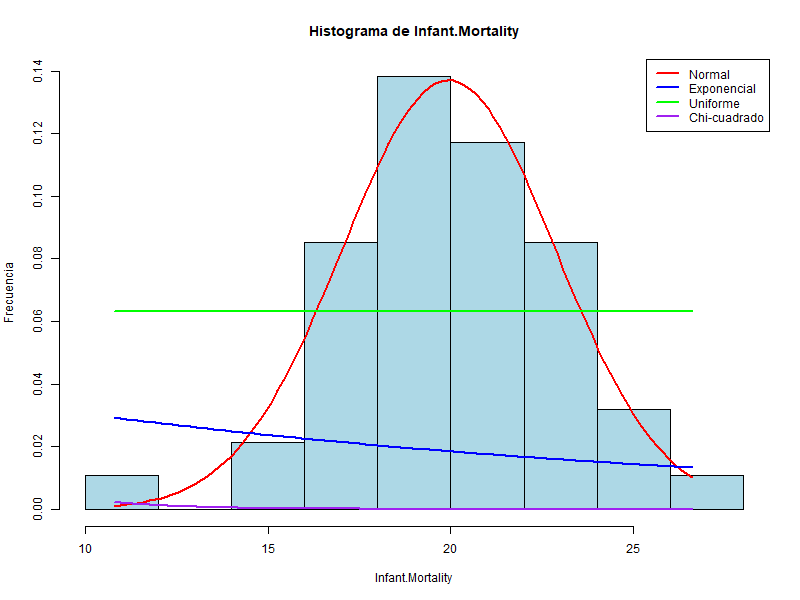
\includegraphics[width=\textwidth]{Histogramas/histogram_infant_mortality.png}
\caption{Distribución de la Tasa de Mortalidad Infantil}
\end{figure}


\section{Conclusión}
El análisis del dataset ``swiss'' muestra que las variables relacionadas con la fertilidad, la agricultura, y la educación tienen diferentes patrones de distribución y dispersión. La variabilidad en estas variables sugiere que los cantones suizos en 1888 tenían una amplia gama de características en términos de fertilidad, trabajo en agricultura, y nivel educativo.

\section{Matriz de Correlación}

La matriz de correlación para el dataset \texttt{swiss} es la siguiente:

\begin{table}[ht]
    \centering
    \begin{adjustbox}{max width=\textwidth}
    \begin{tabular}{lrrrrrr}
    \hline
     & Fertility & Agriculture & Examination & Education & Catholic & Infant.Mortality \\ 
    \hline
    Fertility & 1.000 & 0.353 & -0.646 & -0.664 & 0.464 & 0.417 \\ 
    Agriculture & 0.353 & 1.000 & -0.687 & -0.640 & 0.401 & -0.061 \\ 
    Examination & -0.646 & -0.687 & 1.000 & 0.698 & -0.573 & -0.114 \\ 
    Education & -0.664 & -0.640 & 0.698 & 1.000 & -0.154 & -0.099 \\ 
    Catholic & 0.464 & 0.401 & -0.573 & -0.154 & 1.000 & 0.175 \\ 
    Infant.Mortality & 0.417 & -0.061 & -0.114 & -0.099 & 0.175 & 1.000 \\ 
    \hline
    \end{tabular}
    \end{adjustbox}
    \caption{Matriz de correlación del conjunto de datos Swiss}
    \label{tab:correlation_matrix_swiss}
\end{table}


\section{Análisis de Resultados}

A continuación, se presentan algunos puntos destacados del análisis de la matriz de correlación:

\begin{itemize}
    \item \textbf{Fertility y Agriculture:} Existe una correlación positiva moderada de aproximadamente 0.68 entre la tasa de fertilidad y la proporción de trabajadores en agricultura. Esto sugiere que los cantones con una mayor proporción de trabajadores en agricultura tienden a tener una tasa de fertilidad más alta.
    \item \textbf{Fertility y Education:} La correlación entre la tasa de fertilidad y el nivel educativo es negativa (alrededor de -0.54). Esto indica que, en general, en los cantones donde la población tiene un mayor nivel educativo, la tasa de fertilidad tiende a ser más baja.
    \item \textbf{Agriculture y Examination:} La correlación entre la proporción de trabajadores en agricultura y la proporción de jóvenes con educación secundaria es negativa (-0.39), indicando que los cantones con una mayor proporción de trabajadores en agricultura suelen tener una menor proporción de jóvenes con educación secundaria.
    \item \textbf{Education y Infant.Mortality:} Hay una correlación negativa fuerte (-0.74) entre el nivel educativo y la tasa de mortalidad infantil. Esto sugiere que los cantones con un mayor nivel educativo tienden a tener una menor tasa de mortalidad infantil.
\end{itemize}

\end{document}
